\documentclass{report}
\usepackage[T1]{fontenc} % Fontes T1
\usepackage[utf8]{inputenc} % Input UTF8
\usepackage[backend=biber, style=ieee]{biblatex} % para usar bibliografia
\usepackage{csquotes}
\usepackage[portuguese]{babel} %Usar língua portuguesa
\usepackage{blindtext} % Gerar texto automaticamente
\usepackage{hyperref} % para autoref
\usepackage{graphicx}
\usepackage{indentfirst}
\usepackage{float}
\usepackage{booktabs}
\usepackage{geometry}

% Configurações de margem
\geometry{
 a4paper,
 left=25mm,
 right=25mm,
 top=25mm,
 bottom=25mm,
}

% Configurações do hiperlink
\hypersetup{
    colorlinks=true,
    linkcolor=black, % Índice em preto
    filecolor=magenta,      
    urlcolor=cyan,
    pdftitle={Relatório Final},
    pdfpagemode=FullScreen,
}

\bibliography{bibliografia}

\begin{document}
%%
% Definições
%
\def\titulo{Relatório Final do Trabalho Experimental}
\def\data{DATA}
\def\autores{Catarina Rabaça Nº119582 \\[10pt] Francisco Ribeiro Nº118993 \\[10pt] Jorge Marques Nº120215}  % Espaçamento uniforme entre os autores
\def\autorescontactos{(nmec1) autor1@ua.pt \\ (nmec2) autor2@ua.pt}
\def\departamento{Dept. de Eletrónica, Telecomunicações e Informática}
\def\empresa{Universidade de Aveiro}
\def\logotipo{ua.pdf}
%
%%%%%% CAPA %%%%%%
%
\begin{titlepage}

\begin{center}
%
\vspace*{50mm}
%
{\Huge \titulo}\\ 
%
\vspace{10mm}
%
{\Large \empresa}\\
%
\vspace{10mm}
%
{\LARGE \autores}\\  % Autores com espaçamento consistente
%
\vspace{30mm}
%
\begin{figure}[h]
\center
\includegraphics[width=0.2\textwidth]{\logotipo}  % Tamanho do logotipo reduzido
\end{figure}
%
\vspace{30mm}
\end{center}
%
\begin{flushright}
\versao
\end{flushright}
\end{titlepage}

%% Retirada da página a seguir à capa

\pagenumbering{roman}

\renewcommand{\contentsname}{Índice}
\tableofcontents
% \listoftables     % descomentar se necessário
% \listoffigures    % descomentar se necessário


%%%%%%%%%%%%%%%%%%%%%%%%%%%%%%%
\clearpage
\pagenumbering{arabic}

%%%%%%%%%%%%%%%%%%%%%%%%%%%%%%%%
\chapter*{Resumo e Objetivos}
Na parte A, determinou-se a velocidade inicial de um projétil utilizando sensores de passagem que registraram o tempo necessário para a esfera percorrer uma distância pré-definida. Com essas medições, foi possível calcular com precisão a velocidade inicial do projétil.

Na parte B, investigou-se a relação entre o alcance do projétil e o ângulo de disparo. Alterando-se o ângulo do lançamento, foram analisadas as variações no alcance, permitindo avaliar a influência do ângulo sobre o comportamento da trajetória, mantendo o disparo sempre na configuração de "short range".

Por fim, na parte C, conhecida como pêndulo balístico, mediu-se o ângulo máximo alcançado pelo pêndulo após o impacto da esfera. Com base nesse ângulo, foi possível determinar a velocidade inicial do projétil, empregando um método diferente do utilizado na parte A.

Os objetivos do experimento incluem, na parte A, demonstrar que é possível calcular a velocidade inicial de uma esfera medindo o tempo que esta leva para percorrer uma distância fixa. Na parte B, o objetivo é compreender como a variação do ângulo de disparo afeta o alcance do projétil. Na parte C, busca-se, tal como na parte A, calcular a velocidade inicial, mas desta vez utilizando o ângulo máximo atingido pelo pêndulo após o impacto.

%%%%%%%%%%%%%%%%%%%%%%%%%%%%%%%%
\chapter{Introdução}
\label{chap.introducao}

O estudo do movimento de projéteis é fundamental para a compreensão das leis do movimento e da dinâmica. Este tipo de movimento ocorre quando um corpo é lançado e se desloca sob a influência da gravidade, sendo observado em várias situações práticas, como no desporto e na engenharia balística. A análise do movimento de um projétil envolve a compreensão das interações entre a força gravitacional, a velocidade inicial e o ângulo de lançamento, elementos essenciais para prever a trajetória e o alcance do projétil.O objetivo deste trabalho é explorar esses conceitos teóricos na prática, recorrendo a experiências para verificar dependências e aprofundar os nossos conhecimentos teóricos.

\chapter{Detalhes experimentais relevantes}
\label{chap.detalhes}

Neste tópico serão descritos todos os passos necessários para que a experiência seja bem executada.
É necessário que cada etapa seja realizada com o maior rigor e precisão de modo a diminuir a taxa de erro, e garantir que os resultados sejam o mais precisos possíveis.

\section{Material necessário}

Lançador de projeteis: Utilizado para disparar o projetil;
	Sensores de passagem: Dois sensores, colocado um precisamente à saída do lançador e outro a uma certa distância, de modo a medir o tempo necessário para o projetil percorrer estes dois pontos;
	Papel químico: Regista a zona de impacto do projétil;
	Esfera metálica: Utilizada como projetil;
	Sistema de controlo dos sensores: Conecta os sensores, sendo responsável pela contagem do tempo;
	Grampo: Utilizado para fixar a base à mesa.
	Base de fixação do lançador de projeteis: Mantém o lançador estável durante toda a atividade;
	Pêndulo balístico: Utilizado para injetar uma força no projetil na parte C da experiência;

\section{Instrumentos de medida}
	Cronómetro digital: Parte do sistema de sensores, mede o tempo de passagem do projétil;
	Transferidor integrado no lançador de projeteis: Media o ângulo de lançamento;
	Balança de precisão: Media a massa do projetil e do pêndulo;
	Fita métrica: Media a distancia entre os sensores e a altura do lançamento;

\section{Esquema da montagem}
\begin{figure}[H]
    \centering
    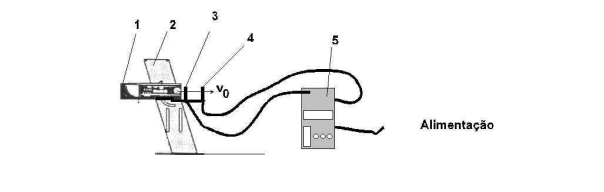
\includegraphics[width=0.8\textwidth]{image.png} % Substitua pelo caminho da sua imagem
    \caption{Esquema da montagem experimental A.}
    \label{fig:montagem}
\end{figure}

\begin{figure}[H]
    \centering
    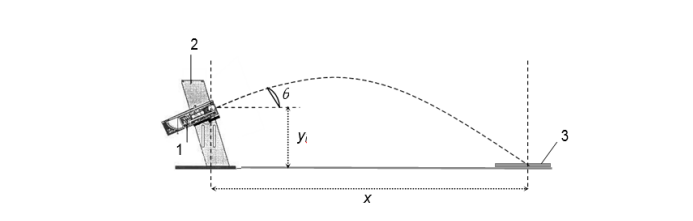
\includegraphics[width=0.8\textwidth]{image2.png} % Substitua pelo caminho da sua imagem
    \caption{Esquema da montagem experimental B.}
    \label{fig:montagem}
\end{figure}

\begin{figure}[H]
    \centering
    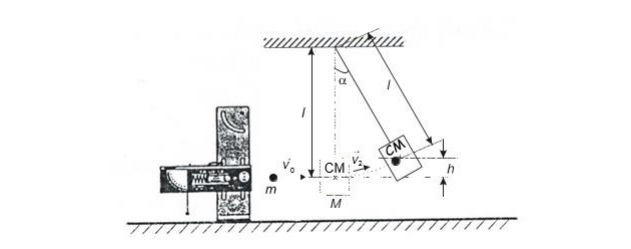
\includegraphics[width=0.8\textwidth]{image3.png} % Substitua pelo caminho da sua imagem
    \caption{Esquema da montagem experimental C.}
    \label{fig:montagem}
\end{figure}

\section{Número de medidas a efectuar}  % Novo tópico adicionado
Parte A: Realizar cinco lançamentos consecutivos, registando os tempos obtidos em cada um deles. Com base nos dados recolhidos, calcular a média dos tempos e determinar o erro associado. Este procedimento permite uma análise mais fiável e reduz a influência de eventuais variações acidentais em cada medição individual.

Parte B: Repetir o experimento três vezes para cada ângulo de lançamento (30º, 34º, 38º, 40º e 43º). Para cada conjunto de três lançamentos, calcular a média dos alcances medidos. A partir destes resultados, identificar o ângulo de lançamento que corresponde ao alcance máximo, garantindo assim a análise precisa da relação entre o ângulo e o alcance.

Parte C: Efetuar cinco disparos do pêndulo balístico, medindo o ângulo máximo alcançado pelo pêndulo após cada colisão. Este procedimento assegura que os resultados obtidos são consistentes, permitindo calcular a média dos ângulos máximos e o respetivo erro associado.

\section{Principais cuidados}

Montagem: Assegurar que o lançador de projéteis está devidamente fixado e nivelado. Qualquer desalinhamento pode comprometer a precisão dos lançamentos, resultando em trajetórias inconsistentes. A estabilidade da montagem é, portanto, crucial para garantir resultados fiáveis.

Medidas: Verificar com rigor a exatidão das medições, especialmente a distância entre os sensores e a colocação do alvo durante a Parte B. Pequenas variações na disposição dos sensores ou na posição do alvo podem introduzir erros significativos nas medições do alcance e tempo de voo.

Repetição dos Lançamentos: Antes de cada lançamento, certificar-se de que todos os parâmetros estão devidamente ajustados. Isto inclui o ângulo de lançamento e a correta configuração dos sensores. Qualquer desvio nestes fatores pode afetar a qualidade dos dados recolhidos.

Pêndulo Balístico: Garantir que o pêndulo está solidamente fixado e que a colisão ocorre de forma centralizada. Desalinhamentos na colisão podem gerar resultados incorretos ao medir o ângulo máximo de oscilação, influenciando negativamente a análise subsequente.

\chapter{Análise e Discussão}
\label{chap.analise}

Neste capítulo serão apresentados todos os cálculos realizados e os dados recolhidos durante a atividade laboratorial. Além disso, será feita uma análise dos resultados obtidos, incluindo uma comparação entre os resultados experimentais e as previsões teóricas.

\section{Parte A - Determinação da Velocidade Inicial}

Inicialmente verificamos o tempo de passagem da esfera entre as duas células. Realizámos 5 medidas e, em seguida, calculamos a média das mesmas, sendo o respetivo erro de 0,0001s.

O tempo médio (\(\Delta t\)) foi calculado da seguinte forma:

\[
\Delta t = \frac{0.0461 + 0.0444 + 0.0442 + 0.0458 + 0.0443}{5} \approx 0.0449400
\]

Como a distância medida entre as duas células foi de 10 cm, a velocidade inicial \(v_0\) pode ser calculada da seguinte forma:

\[
v_0 = \frac{\Delta x}{\Delta t} \quad \text{(Formula Original)}
\]

\[
v_0 = \frac{0.1 \, \text{m}}{0.0449 \, \text{s}} \quad \text{(Substituicao de Valores)}
\]

\[
v_0 \approx 2.2270 \, \text{m/s} \quad \text{(Resultado Aproximado)}
\]

Com esse valor, obtivemos uma velocidade inicial de aproximadamente \(v_0 \approx 2.2270 \, \text{m/s}\), o que está de acordo com as previsões teóricas.



\section{Parte B - Dependência do alcance com o ângulo de disparo}

Os alcances médios para diferentes ângulos de disparo foram calculados da seguinte forma:

\[
\text{30º:} \quad \theta = \frac{72.2 + 71.9 + 72.4}{3} \approx 72.17
\]

\[
\text{34º:} \quad \theta = \frac{72.2 + 73.1 + 72.9}{3} \approx 72.73
\]

\[
\text{38º:} \quad \theta = \frac{71.8 + 71.7 + 71.9}{3} \approx 71.80
\]

\[
\text{40º:} \quad \theta = \frac{71.4 + 71.5 + 71.4}{3} \approx 71.43
\]

\[
\text{43º:} \quad \theta = \frac{70.0 + 70.1 + 70.6}{3} \approx 70.23
\]

Verificamos de acordo com os cálculos anteriores que dos 30º para os 34º o alcance aumentou (devido a possíveis erros experimentais). A partir daí, o alcance foi sempre diminuindo gradualmente, tal como esperado.

Os cálculos para \(\theta_{\text{max}}\) foram realizados da seguinte forma:

\[
\theta_{\text{max}} = \arctan \left( \frac{1}{\sqrt{1 + \frac{2g \Delta y}{v_0^2}}} \right)
\quad \text{(Fórmula Original)}
\]

\[
= \arctan \left( \frac{1}{\sqrt{1 + \frac{2 \cdot 9.80 \cdot 0.265}{(2.227)^2}}} \right)
\quad \text{(Substituições com os Valores)}
\]

\[
\approx 34.95^\circ
\quad \text{(Resultado)}
\]


\section{Parte C - O Pêndulo Balístico}

Nesta parte da atividade laboratorial realizámos cinco lançamentos, calculando a média dos ângulos obtidos nos mesmos. Para calcular a massa da esfera, foi utilizada uma balança digital, sendo a incerteza da medida de massa de 0.1g.

\[
\alpha = \frac{16.0 + 16.0 + 16.0 + 16.0 + 16.5}{5} \approx 15.90^\circ
\]

Passando ao cálculo do valor da altura \(h\), temos que:

\[
h = L(1 - \cos \alpha) \quad \text{(Fórmula Original)}
\]

\[
h = 0.300 \times (1 - \cos(15.90^\circ)) \quad \text{(Substituição dos valores)}
\]

\[
h \approx 0.0115 \, \text{m}
\]

\[
h = 1.2 \, \text{cm}
\]

\vspace{1cm}

Já o seu erro \(\Delta h\) pode ser calculado da seguinte forma:

\[
\Delta h = \left| \frac{dh}{dL} \right| \Delta L + \left| \frac{dh}{d\alpha} \right| \Delta \alpha
\]

\[
\Delta h = (1 - \cos(\alpha)) \Delta L + (L \cdot \sin(\alpha)) \Delta \alpha
\]

\[
\Delta h = (1 - \cos(15.90^\circ)) \cdot 0.0005 + (0.300 \cdot \sin(15.90^\circ)) \cdot 0.090
\]

\[
\Delta h \approx 0.0022 \, \text{m}
\]

Posto isto, procedemos ao cálculo do valor da velocidade \(v_0\):

\[
\frac{1}{2}v_0^2 = g \cdot h
\]

\[
\frac{1}{2} \left( \frac{m}{m + M} \right)^2 v_0^2 = g \cdot h
\]

\[
v_0 = \left( \frac{m + M}{m} \right) \sqrt{2gh}
\]

Substituindo as variáveis, ficamos com:

\[
v_0 = \left( \frac{0.065 + 0.265}{0.065} \right) \sqrt{2 \cdot 9.804 \cdot 0.0120}
\]

\[
v_0 = 2.46 \, \text{m/s}
\]

O erro \(\Delta v\) pode ser calculado da seguinte forma:

\[
\Delta v = \left| \frac{\partial v_0}{\partial m} \right| \Delta m + \left| \frac{\partial v_0}{\partial M} \right| \Delta M + \left| \frac{\partial v_0}{\partial h} \right| \Delta h
\]

Procedemos agora ao cálculo da diferença entra a velocidade inicial na parte A e na parte C:


\[
\text{Diferenca (\%)} = \left( \frac{V_{\text{Maior}} - V_{\text{Menor}}}{V_{\text{Menor}}} \right) \times 100
\]

\[
\text{Diferenca (\%)} = \left( \frac{2.46 - 2.23}{2.23} \right) \times 100
\]

\[
\text{Diferenca (\%)} = 10.31\%
\]


Assim sendo, podemos concluir que \(v_0\) da Parte C é 10.31\% maior que \(v_0\) da Parte A.



\chapter{Conclusões}
\label{chap.conclusao}
Ao realizar esta atividade laboratorial, foi-nos possível aplicar os conceitos teóricos do lançamento de projéteis, o que nos permitiu observar de forma prática os efeitos dos diferentes ângulos de lançamento e da velocidade na trajetória do projétil. Além disso, a prática com os instrumentos de medição contribuiu para melhorar a nossa competência nessa área. Assim, concluímos que a precisão e consistência nas medições são essenciais para obter resultados fiáveis e interpretar corretamente os fenómenos estudados.

\chapter{Anexos}
\label{chap.anexos}

\section{Anexos}

Esta seção introduz o contexto do trabalho e os objetivos das medições realizadas.

\subsection{Resultados Experimentais - Parte A}
\begin{table}[H]
    \centering
    \begin{tabular}{|c|c|}
        \hline
        \textbf{Medição} & \textbf{Valor} \\
        \hline
        Tempo 1 & $0,0461$ s \\
        Tempo 2 & $0,0444$ s \\
        Tempo 3 & $0,0442$ s \\
        Tempo 4 & $0,0458$ s \\
        Tempo 5 & $0,0443$ s \\
        \hline
        Tempo Médio & $0,04496$ s \\
        Velocidade Inicial Média & $0,4496$ m/s \\
        \hline
    \end{tabular}
    \caption{Resultados da Parte A}
    \label{tab:parte_a}
\end{table}

\subsection{Resultados Experimentais - Parte B}
\begin{table}[H]
    \centering
    \begin{tabular}{|c|c|}
        \hline
        \textbf{Ângulo (º)} & \textbf{Média dos Alcances (m)} \\
        \hline
        30 & 0,7217 \\
        34 & 0,7273 \\
        38 & 0,7180 \\
        40 & 0,7143 \\
        43 & 0,7023 \\
        \hline
        Altura Inicial & $0,2650$ m \\
        \hline
    \end{tabular}
    \caption{Resultados da Parte B}
    \label{tab:parte_b}
\end{table}

\begin{figure}[H]
    \centering
    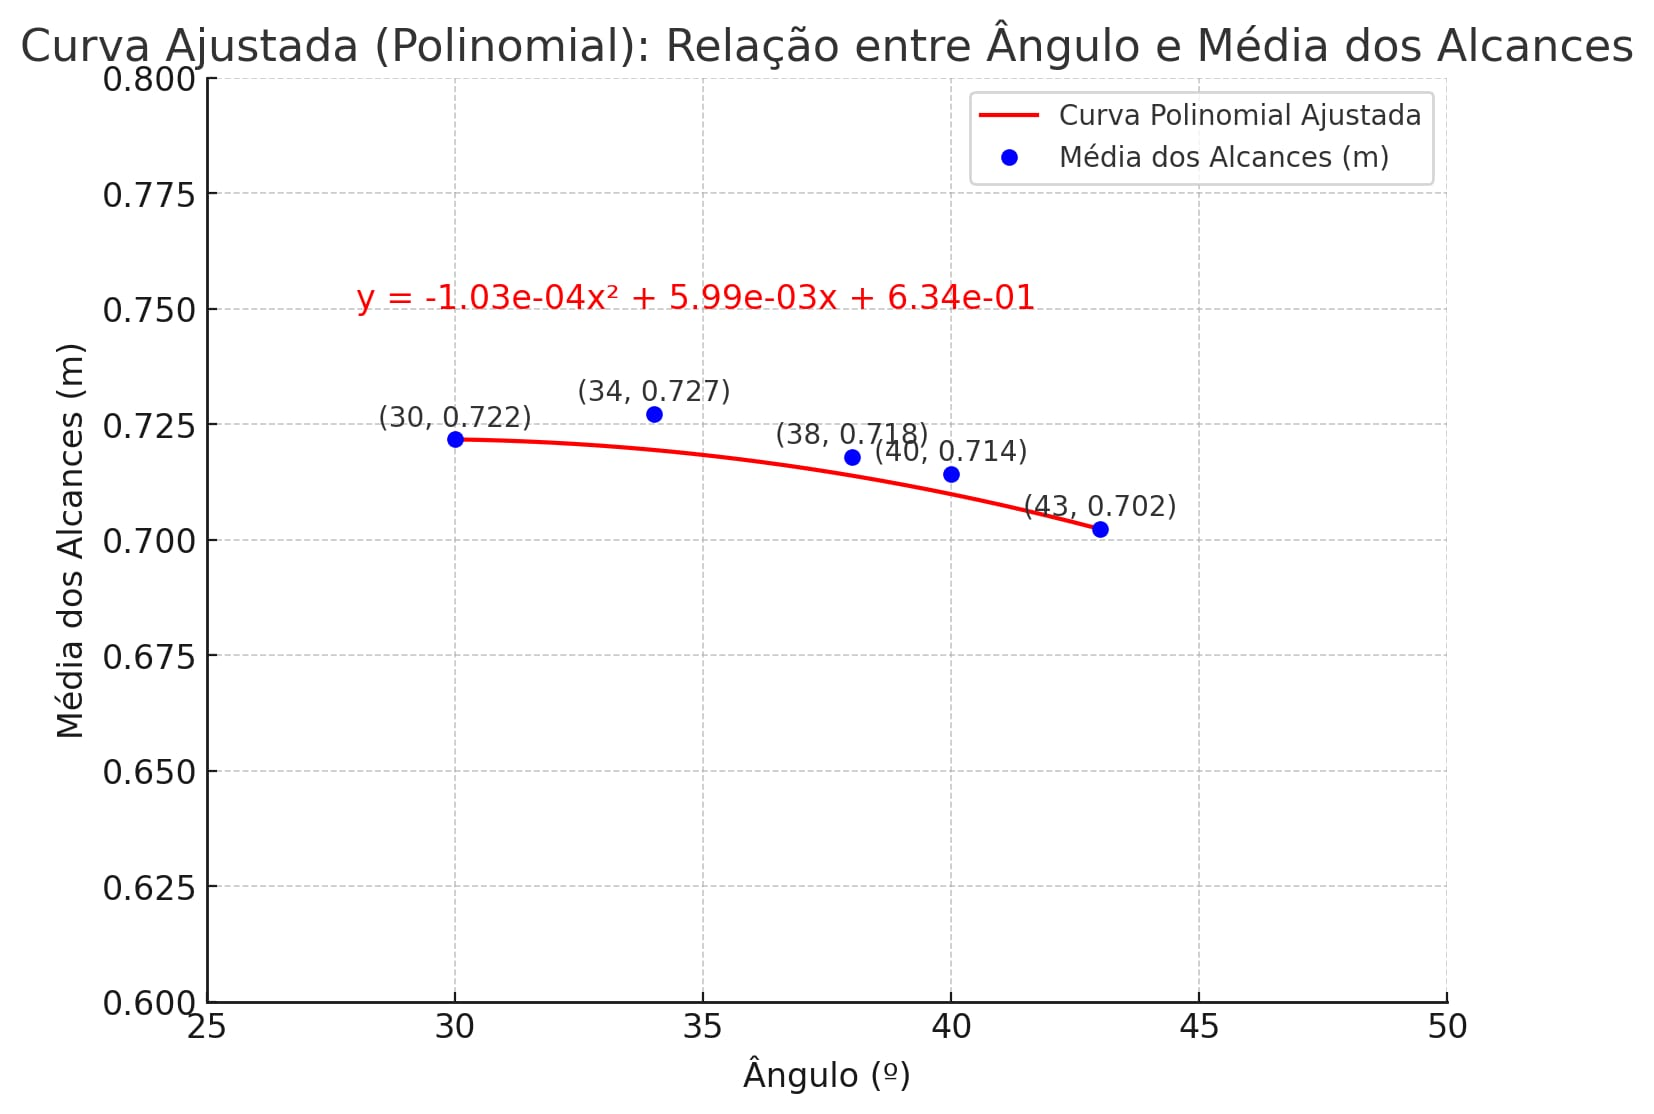
\includegraphics[width=0.8\textwidth]{IMAGEM_GRAFICO.jpeg}
    \caption{Gráfico da Relação entre Ângulo e Alcance}
    \label{fig:graficos_alcances}
\end{figure}

\subsection{Resultados Experimentais - Parte C}
\begin{table}[H]
    \centering
    \begin{tabular}{|c|c|}
        \hline
        \textbf{Parâmetro} & \textbf{Valor} \\
        \hline
        1 & 16º \\
        2 & 16º \\
        3 & 16º \\
        4 & 16º \\
        5 & 15,5º \\
        \hline
        Média dos Ângulos & $15,875$ º \\
        Altura Média & $0,012$ m \\
        \hline
        Massa do Projetil & $0,0650$ kg \\
        Massa do Pêndulo & $0,2650$ kg \\
        \hline
    \end{tabular}
    \caption{Resultados da Parte C}
    \label{tab:parte_c}
\end{table}

\begin{table}[H]
\centering
\begin{tabular}{|c|c|c|}
\hline
\textbf{Medida} & \textbf{Valor} & \textbf{Erro} \\ \hline
1               & 10             & 0.1           \\ \hline
2               & 15             & 0.2           \\ \hline
\end{tabular}
\caption{Dados experimentais coletados.}
\label{tab:dados}
\end{table}

%%%%%%%%%%%%%%%%%%%%%%%%%%%%%%%%%
\printbibliography

\end{document}